% NOTES 
% Wie ich den sprinback gemssen habe 

\chapter{Build}

\section{Problem Statement}
The following design principles is a selection of \cite{siebert_constructionqualitymodel_}'s quality parameters for \ac{ML} models.
In this \ac{DSR} work the artifacts are \ac{ML} models therefore these design principles are used to evaluate them.

\subsubsection*{Design Principle 1: Correctness}
\textit{Does the artifact predict the spring back of a sheet metal with a high accuracy and correctness?}
With progression in manufacturing there is a growing demand for high-quality products, that means that the meta parts needs to be produced with high precision and accuracy. Here the sprin back is an undesired side effect which need to be mimimized. \cite[p. 1]{baig_machinelearningprediction_2021}
Sheet metal forming in manufacturing need a high level of quality and precision. Therefore, the spring back of a sheet metal is an important parameter to consider. \cite[p. 1]{cruz_applicationmachinelearning_2021}
Predicting spring back is important to reduce the number of trial and error cycles in the manufacturing process.
Also predicting spring back is complex because of many variables and parameters and often not all of them are known.
Therefore, a machine learning model should predict the spring back of a sheet metal with a high accuracy and correctness. When using the \ac{ML} model small errors in the prediction can cause fitting problems in the manufacturing process.

% Using an analytical model to compare the artifact. (miranda 2018 paper)

\subsubsection*{Design Principle 2: Appropriateness}
\textit{Is the artifact appropriate for the given problem?}
While selecting a model it is important that it fits the problem/task and can deal with the given data. \cite[p. 16]{siebert_constructionqualitymodel_}


\subsubsection*{Design Principle 3: Relevance}
\textit{Does the artifact achieve a good bias-variance trade-off?}

In addition to measure the correctness it is important to understand "why" the learner has this performance.
This is important to understand the limitations of the model and to improve it.
Therefore, it is important to understand the bias-variance trade-off. \cite[p. 50]{zhou_machinelearning_2021}
Bias measures the differences between the learnesrs expected prediction and the ground-truth label. This results in the fitting ability of the learner.
Variances measures the change of learning performance of the learner because of changes in the training set. This results in the impact of data disturbance on the results. \cite[p. 51]{zhou_machinelearning_2021}

\subsubsection*{Design Principle 4: Robustness}
\textit{How well does the artifact handle outliers, noise and missing data?}
Using real-world data noice is a common problem and can have a negative impact on the performance of the learner. Therefore, it is important to measure how good the artifact performs when dealing with impact data.
\cite{saez_evaluatingclassifierbehavior_2016} proposed a new measure to establish the expected behavior of a learner with noisy data trying to minimize the problems: the Equalized Loss of Accuracy (ELA). \cite[p. 3]{saez_evaluatingclassifierbehavior_2016}

\subsubsection*{Design Principle 5: Stability}
\textit{Does the artifact generate repeatable results when trained on different datasets?}


\subsubsection*{Design Principle 6: Interpretability}
\textit{Is the artifact easy to understand and explain?}

It should be noticed, that there are many parameters and variables involved in the sheet metal forming process.
That makes the process design quite complex, particularly in the production of components which require several stages, and thus more than one set of tools. \cite[p. 1]{dib_singleensembleclassifiers_2020}
A model which allows conclusions how the results where generated is better.

\subsection*{Design Principle 7: Resource utilization}
\textit{How many resources does the artifact need to train and predict?}

Conventional processes are often based on empirical trial and error approaches. \cite[p. 1]{dib_singleensembleclassifiers_2020}
A common approach is to experimentally create so named 'technology tables' which contain the bending parameters and the resulting spring back. (Quelle: Hochstrate?)
This process is time and cost intensive and therefore often not suitable for the production of high-volume and low-cost components.
Therefore, one of the benefits of using machine learning should be the reduction of the number of trial and error cycles in the manufacturing process.
Furthermore, training the model should take not too much time and resources.
As mentioned before often FEM-simulation are used to virtually try out metal forming processes. However, fully exploring the design space is computationally expensive and often not possible. \cite[p. 3]{dib_singleensembleclassifiers_2020}
The number of experiments can be reduced using a meta-model like \ac{ANN}. \cite[p. 3]{dib_singleensembleclassifiers_2020}
A approach fully based on \ac{ML} should perfor



\section{Dataset generation}
For the dataset generation, bending experiments were performed on metal sheets with different thicknesses.
% material
The material used is cold rolled steel sheets of the norm DIN EN 10130. The thicknesses used were 0.5mm, 1mmm and 2mm.
The material was used because it is commonly used in bending processes and its high availability. In previous tests, it was observed, that the spring back are well observable with this material.
Using this material, 200 single bending pieces of the dimension 20×100 mm have been cut.
Each piece was bend one time using a \textit{Zwick} three-point-bending machine.

Python script where developed to covert the output data format from the machine to CSV files.
The following describes the experimental setup used for the experiments performed.

\subsection{Preliminary Tests}
A number of preliminary tests were conducted to determine the influence of the punch penetration on the spring back.

\subsubsection{Multiple Cycles}
One approach was to test if multiple spring back can be measure using only one sheet.
Therefore, the machine was programmed to perform multiple cycles in one attempt and bend the metal sheet multiple times. The benefit of this approach would have been a faster generation of the dataset because spring backs could be measured in on attempt, also less material would have been used.

Figure~\ref{springback_multiple} shows one of these attempts. The metal sheet was bent 4 times using $y_p$ values from 5 to 8. The results show, that 4 different spring backs can be measured, but the spring back does not vary like expected. It was observed as well, that the spring backs are different in every attempt, this is shown in Figure~\ref{springback_multiple_inconsistent_results}.
Bending 4 different metal sheets each only one time returned very different results.
A possible explanation could be the cold deformation of the steel, which is not reversible. Because this approach did not work, the machine was programmed to perform one cycle at a time.

\captionsetup{width=0.45\textwidth}

\begin{figure}[H]
    \centering
    \begin{minipage}[b]{0.5\textwidth}
        \centering
        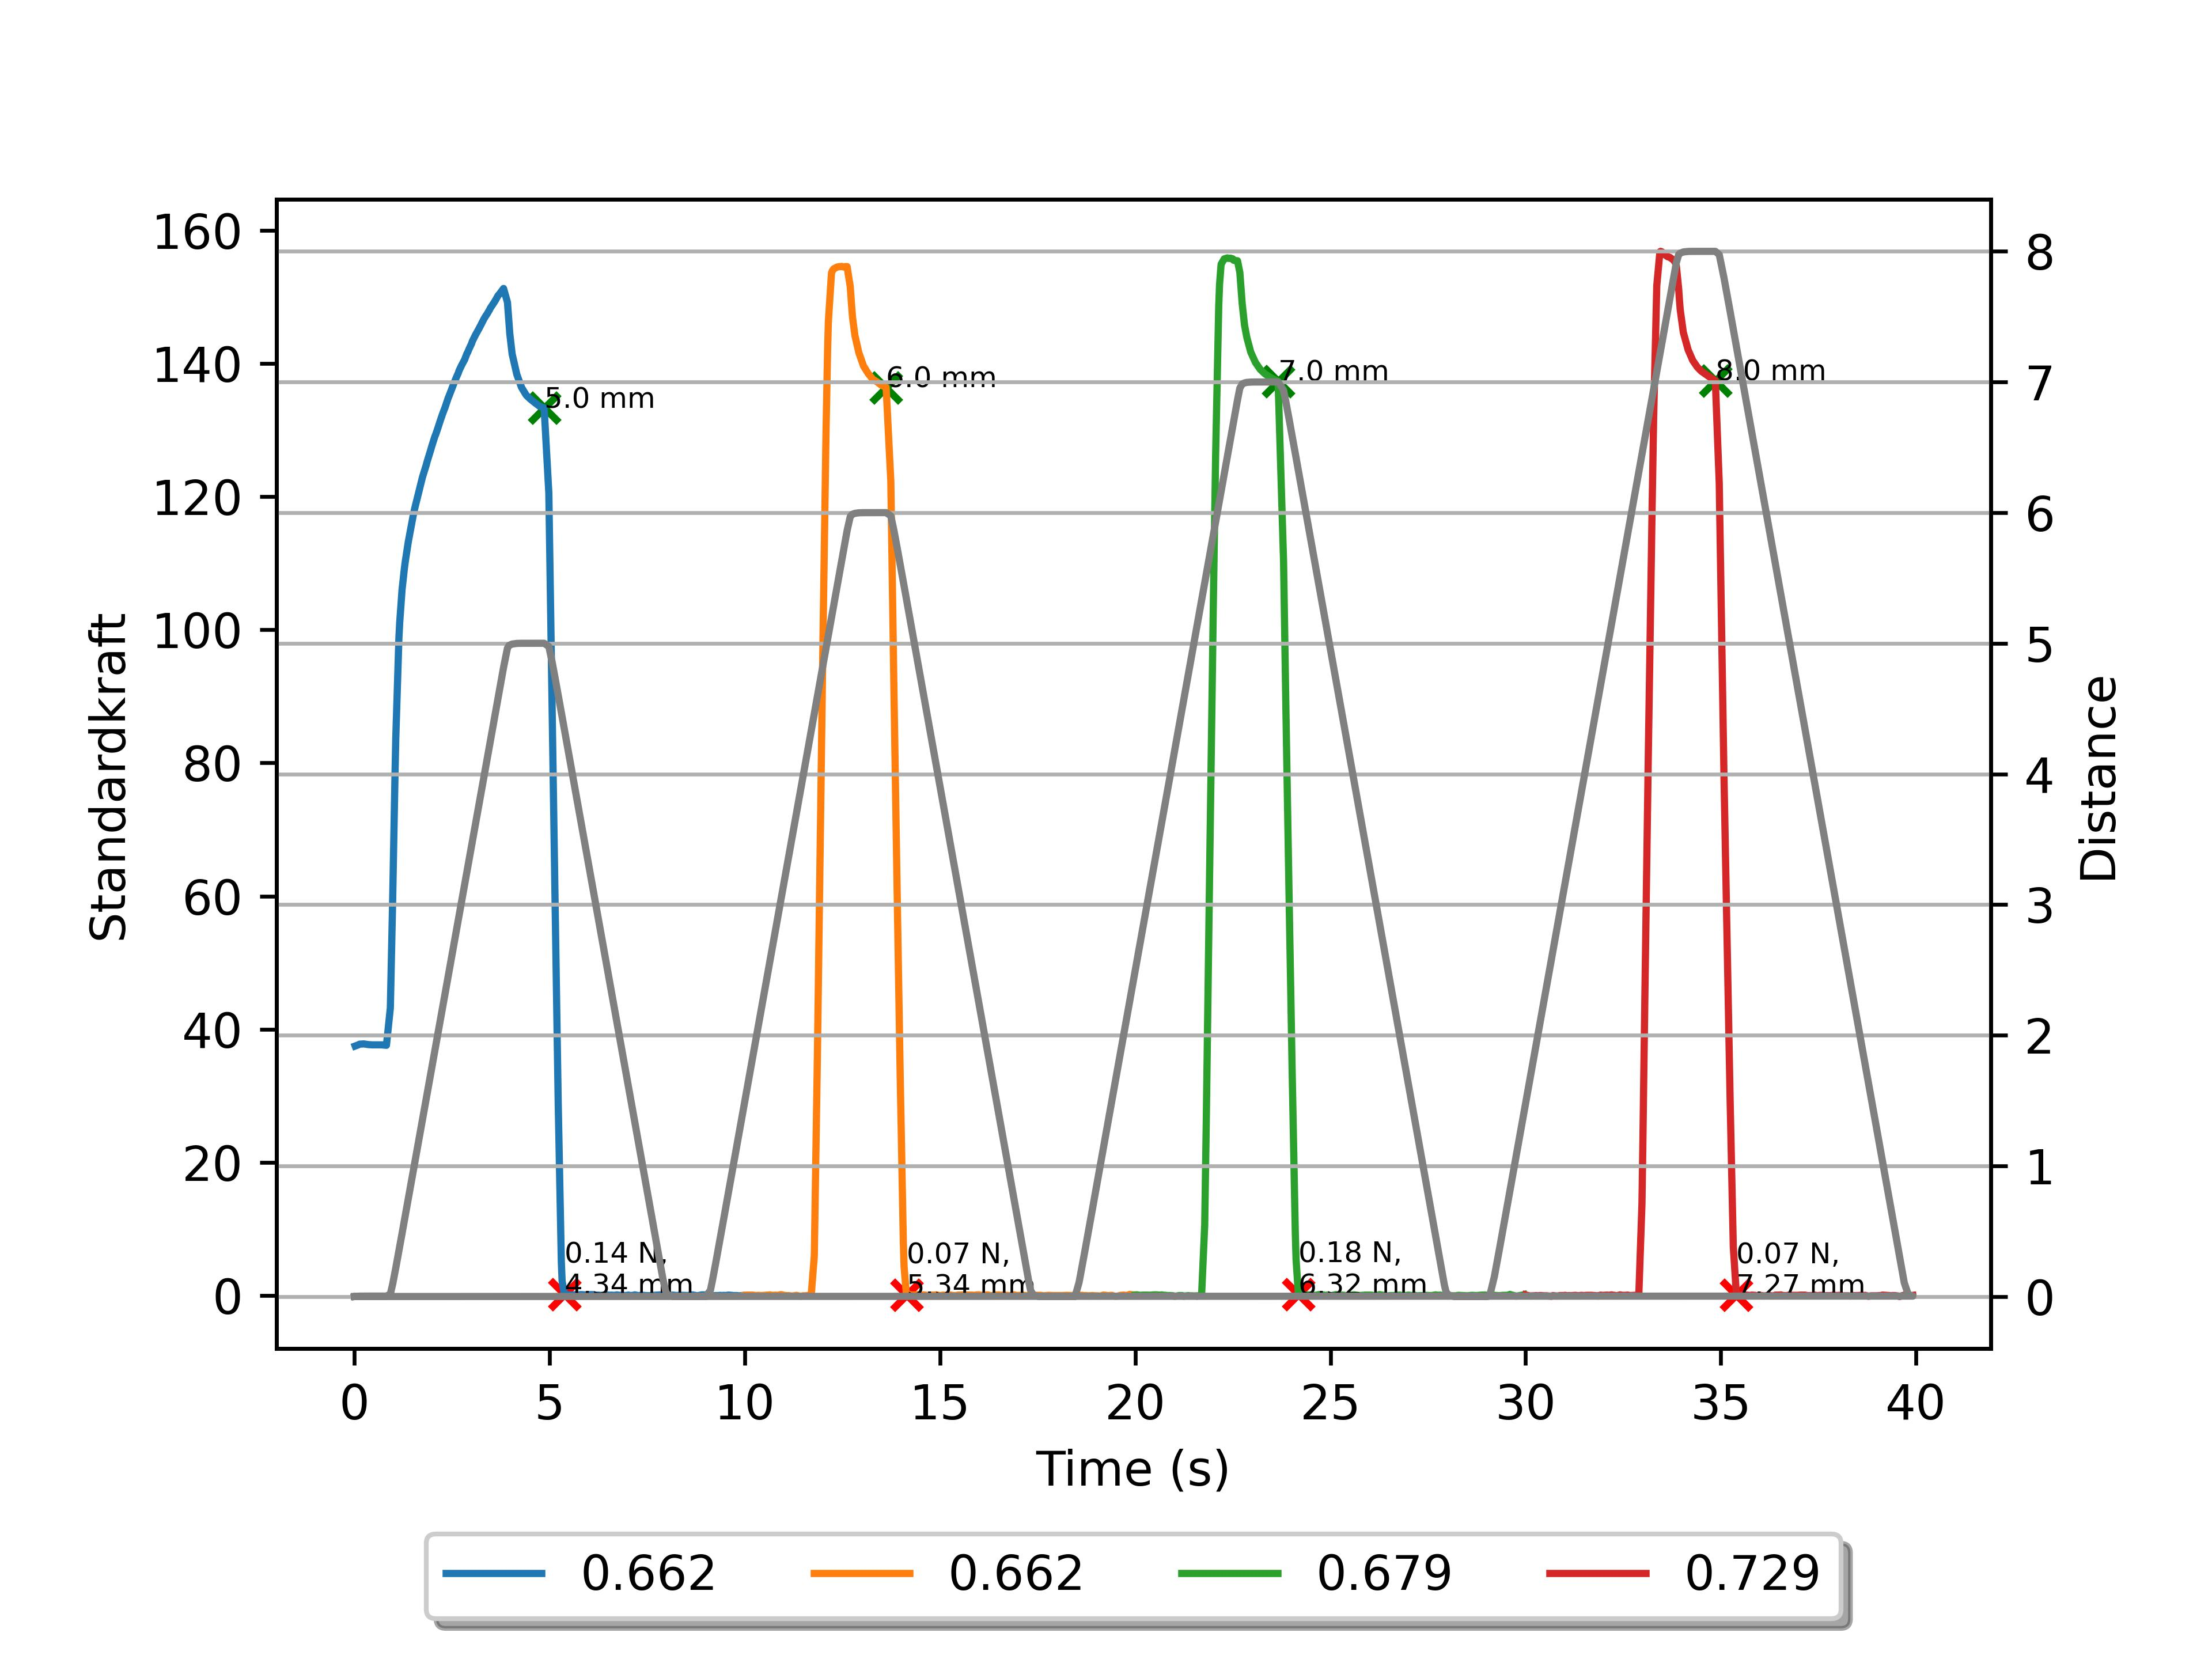
\includegraphics[width=0.9\textwidth]{springback_multiple.jpg} % first figure itself
        \caption{Experiment: Bending one metal sheet multiple times with different $y_p$ values.}
        \label{springback_multiple}
    \end{minipage}\hfill
    \begin{minipage}[b]{0.5\textwidth}
        \centering
        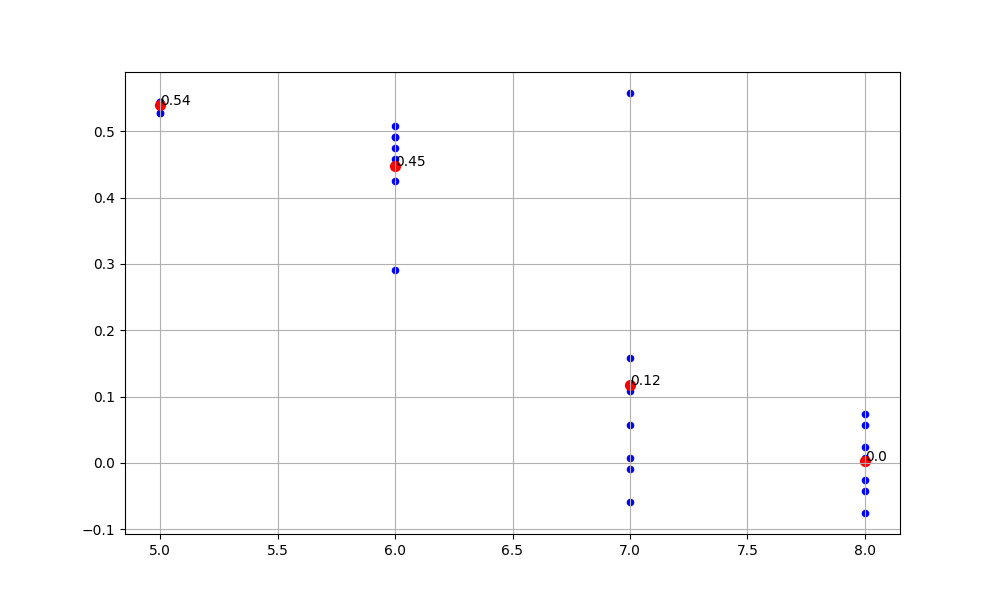
\includegraphics[width=1.1\textwidth]{springback_multiple_inconsistent_results.png} % second figure itself
        \caption{Inconsisten results bending one metal sheet mutliple times. The spread of the results is very large.}
        \label{springback_multiple_inconsistent_results}
    \end{minipage}
    \label{fig:springback_multiple_overview}
\end{figure}

\subsubsection{Brake Bending Machine}
Before using the three point bending machine, a brake bending machine was used to test the influence of the bending on the spring back. The brake bending machine is a machine used to bend metal sheets. It is a very common machine in the industry and is used to bend metal sheets to a specific radius. The brake bending machine used is a \textit{Bendmaster 1000} from \textit{Bendmaster}.

After a series of bends it was observed, that the spring back values where much higher than expected. The explanation for that behavior was, that altering the position the bending beam of that specific machine was not enough to get the desired angle. Thus, the machine excluded for the generation of the data and the three point bending machine was used instead.

Despite the inaccurate data, it was later observed, that the distribution of the spring backs was very similar to the later experiments with the three point bending machine.


\subsection{Experimental setup}
The setup consists of a three-point-bending machine with a punch and a die with no bottom. The machine used is the \textit{Zwick MX 25A} material testing machine.
The machine is equipped with a load cell and a displacement sensor. The load cell is used to measure the force applied to the sheet and the displacement sensor is used to measure the displacement of the punch.
The machine is controlled by a computer and a software called \textit{ZwickRoell TestXpert}. The software is used to control the machine and to save the output data.

The experimental setup and the process parameters are shown in Figure~\ref{fig:setup} where $V$ is the die opening, $y_p$ is the punch penetration which is the distance the punch is moved into the sheet.
The paramter $t$ is the sheet thickness,  $\alpha$ is the sheet corresponding bending angle. Parameter $r_p$ is the punch radius which is the radius of the tip of the punch and $r_m$ is the die radius.


\begin{figure}[H]
    \centering
    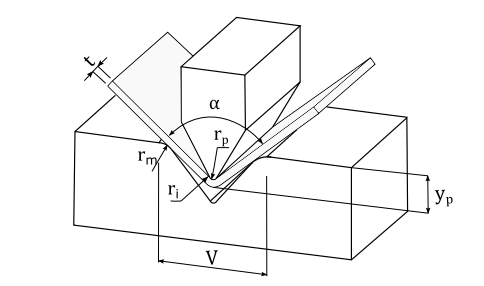
\includegraphics[width=0.6\textwidth]{setup}
    \caption{Process parameters: Sheet bending angle ($\alpha$), sheet thickness ($t$), punch penetration ($y_p$), die opening ($V$), punch radius ($r_p$), die radius ($r_m$), inside bending radius ($r_i$).}
    \label{fig:setup}
\end{figure}

In order to get consistent results, a number of constant and variable parameters were chosen.
The parameters include the punch-and-die tooling made of steel where die punch had a radius ($r_p$) of 5 mm and and die radius ($r_m$) of 10 mm. The die opening $V$ was varied between 10 and 50 mm and the punch penetration $y_p$ was varied between 0 and 20 mm.
The machine was configured to move the punch with a constant speed of 100 mm/min until it measured a resistance of 1 N. That meant, that the punch reached the metal plate and the actual bending process can start. After a hold time of 1 second the punch was moved with a slower speed of 8 mm/min until the specified punch penetration was reached.
The length and width of the metal sheet was 100 mm and 20 mm respectively. The sheet thickness was varied between 0.5 and 3 mm.
The constant parameters are shown in Table~\ref{tab:constant_parameters} and the varying parameters are shown in Table~\ref{tab:varying_parameters}.

\begin{table}[H]
    \centering
    \begin{tabular}{|l|l|l|l|}
        \hline
        \textbf{Parameter} & \textbf{} & \textbf{Value}                      & \textbf{Unit} \\ \hline
        Punch penetration  & $y_p$     & 2.5, 5, 7.5, 10, 12.5, 15, 17.5, 20 & mm            \\
        Die opening        & $V$       & 10, 20, 30, 40, 50                  & mm            \\
        Thickness          & $t$       & 0,5, 1, 1.5, 2, 2.5, 3              & mm            \\
        \hline
    \end{tabular}
    \caption{Experimental setup varying parameters}
    \label{tab:varying_parameters}
\end{table}

\begin{table}[H]
    \centering
    \begin{tabular}{|l|l|l|}
        \hline
        \textbf{Parameter}            & \textbf{Value} & \textbf{Unit} \\ \hline
        Punch radius                  & 5              & mm            \\
        Die radius                    & 5              & mm            \\
        Sheet thickness               & 0.5, 1, 2      & mm            \\
        Sheet width                   & 20             & mm            \\
        Sheet length                  & 100            & mm            \\
        Punch speed                   & 100            & mm/min        \\
        Punch speed after penetration & 8              & mm/min        \\
        Punch force                   & 1              & N             \\
        \hline
    \end{tabular}
    \caption{Experimental setup constant parameters}
    \label{tab:constant_parameters}
\end{table}





\subsection{Measuring The Spring Back} \label{sec:measuring_the_spring_back}
The output data contained different data points, which were used to calculate the spring back.
Important parameters for the calculation are the force, punch penetration and testing time.
As shown in Figure~\ref{fig:springback_measured} at the $yp$ maximum the punch penetration and the force are maximized as well. The punch stays at that position for 1 second and then moves back with a slower speed. This hold time a limitation of the machine and can not be changed.
After the punch is moved back, the force is reduced and the punch penetration is reduced as well, until the punch is at the initial position. For a short time after the lift, the load  cell still measures a force. That is because the metal sheet springs back and the punch is still in contact with the sheet. This was measured using a python script, the green and the yellow point represent the resulting spring back distance.

\begin{figure}[H]
    \centering
    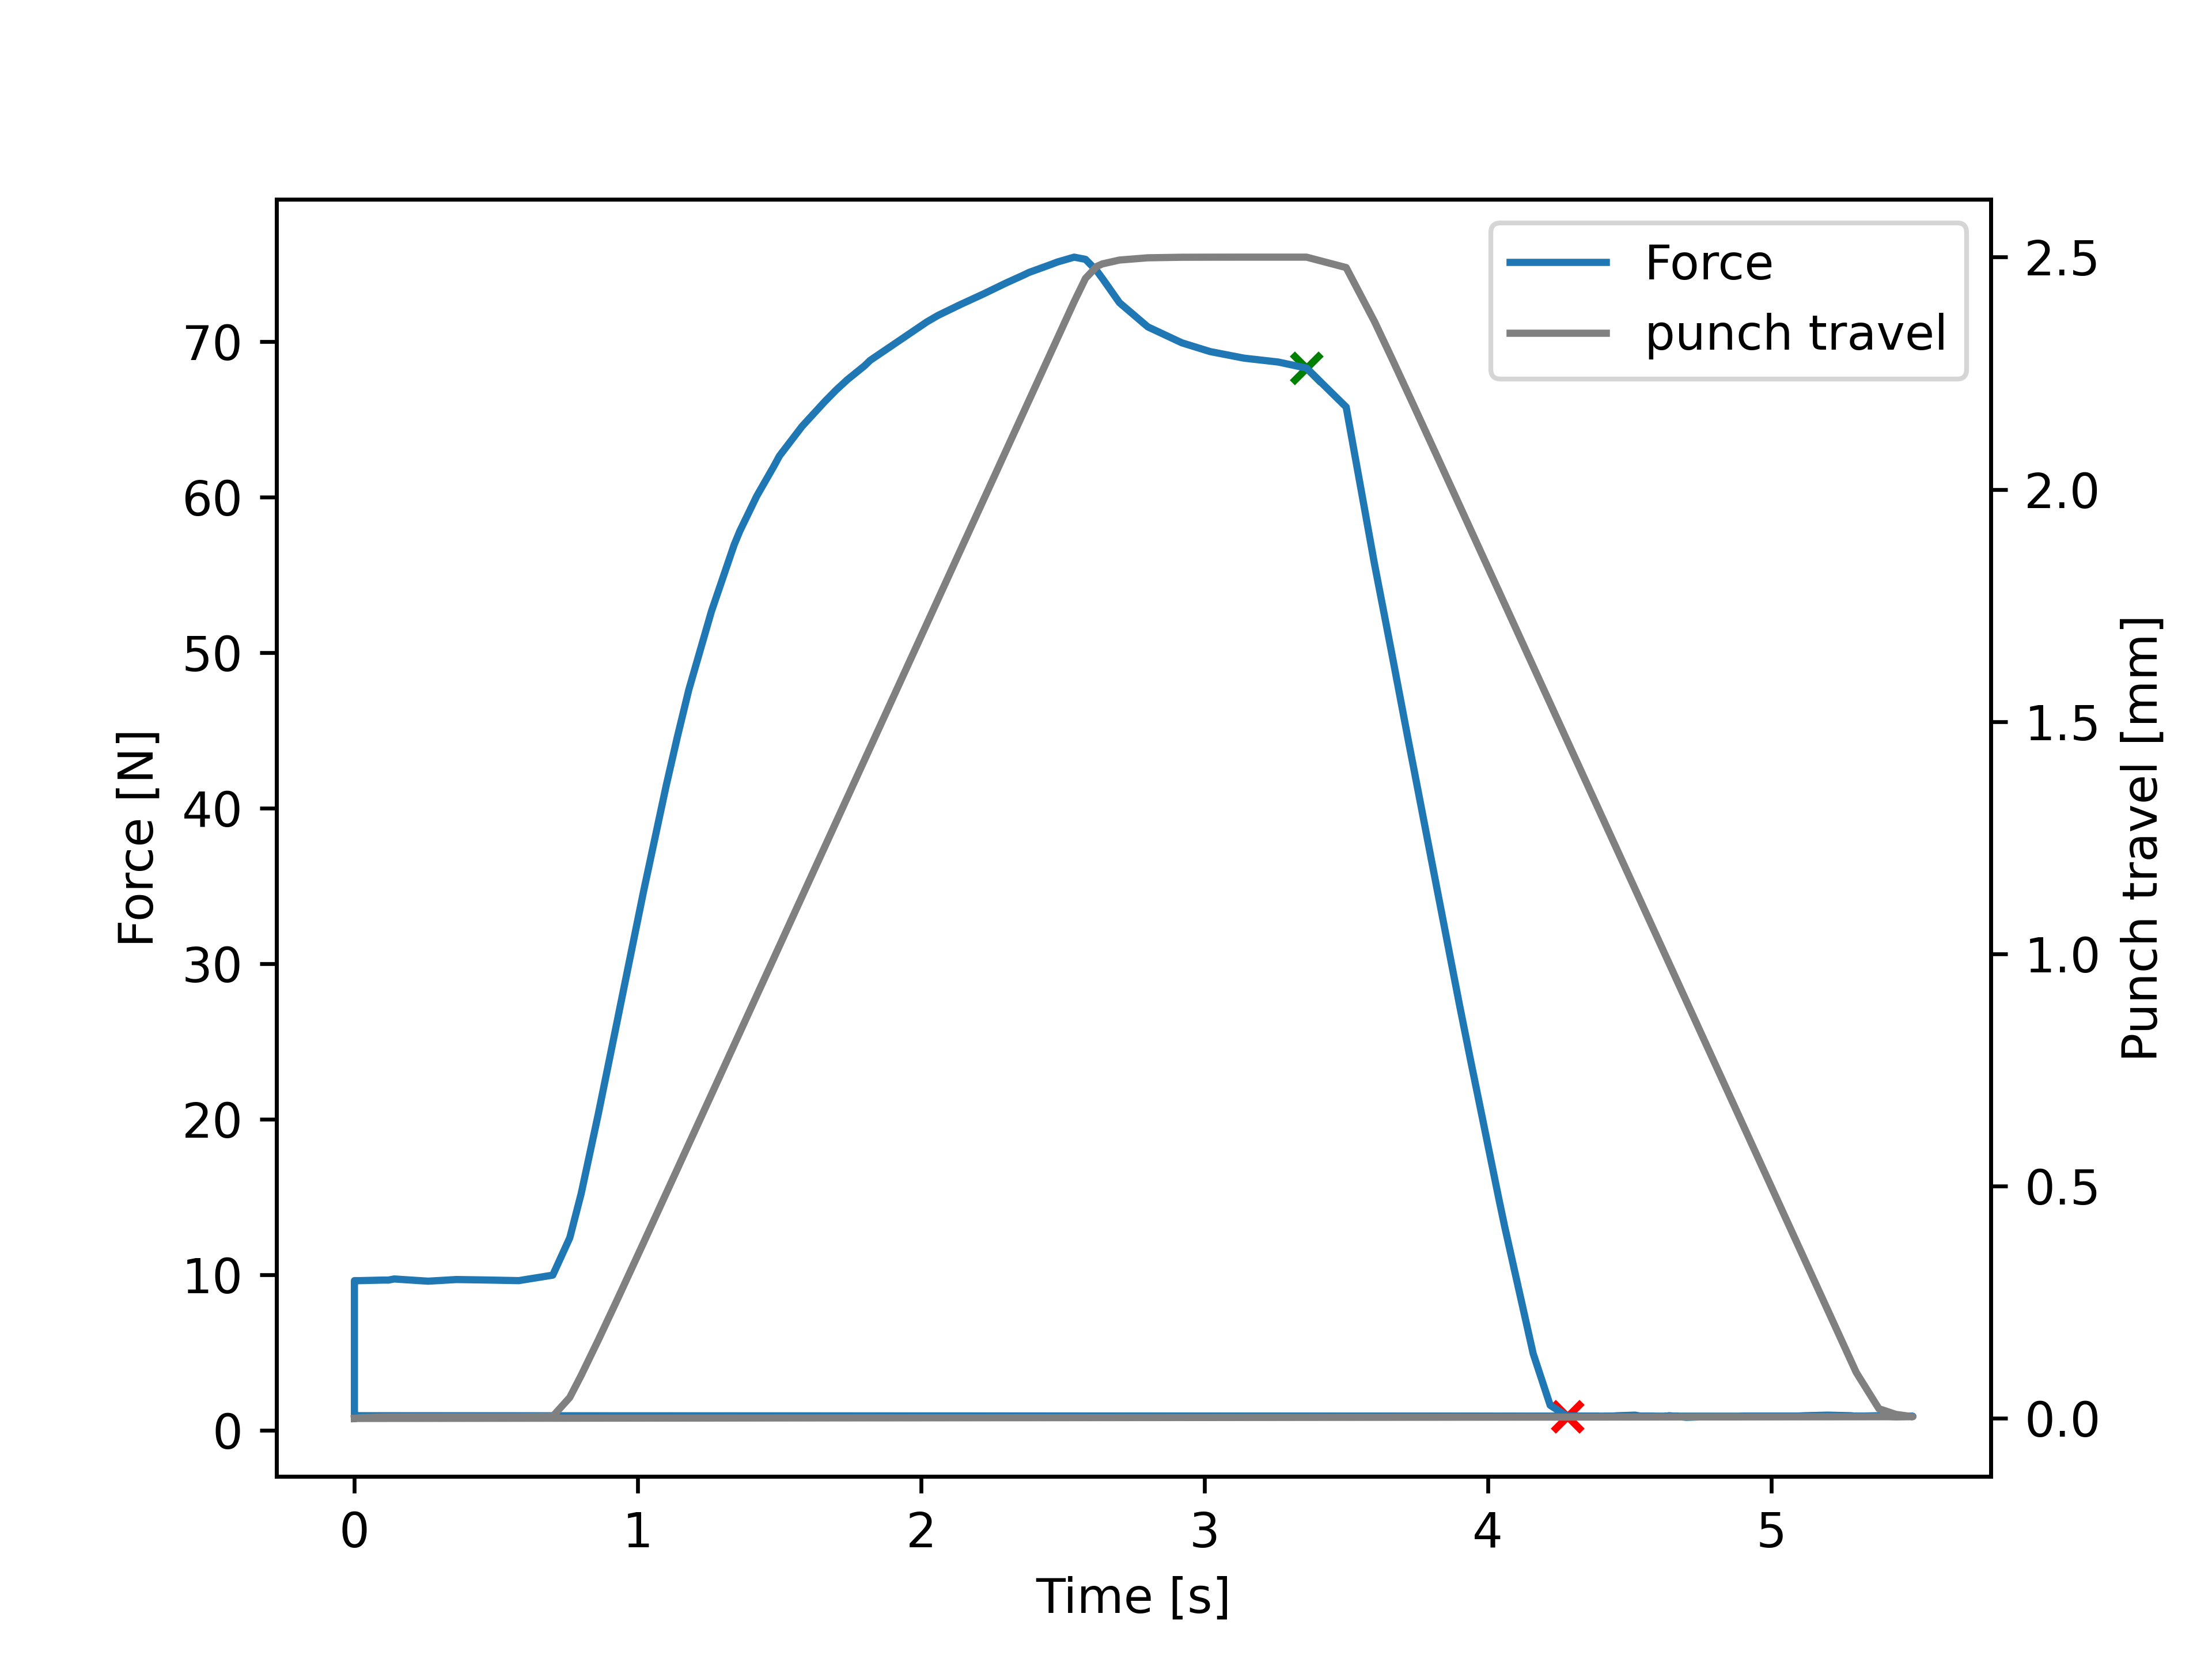
\includegraphics[width=0.7\textwidth]{springback_measured}
    \caption{A steel metal sheet was bent with a punch penetration of 5 mm the spring back is 0.37 mm. The blue line shows the force and the blue line shows the punch penetration.}
    \label{fig:springback_measured}
\end{figure}

\begin{filecontents*}{example.dat}
    Method Pink-1C Pink-AC Green-1C Green-AC Blue-1C Blue-AC Cyan-1C Cyan-AC Red-1C Red-AC Orange-1C Orange-AC
    Square 24.75 4.8 32.28 7.39 32.65 7.53 31.96 7.18 33.57 8 33.19 7.08
\end{filecontents*}

\subsection{Exploring The Dataset}
The output data of the bending machine contained 26 features which can be found in the appendix. Out of these features only the standard power and the distance $y_p$ and the force are relevant for calculating the spring back which was described in the last section \ref{sec:measuring_the_spring_back}.
The final dataset therefore contained 3 features plus the added spring back.
In total 396 data points where crated using the described approach.
An example of the dataset is shown in Table~\ref{tab:dataset_example}.

\begin{table}[H]
    \centering
    \begin{tabular}{|l|l|l|l|l|}
        \hline
        \textbf{} & \textbf{distance} & \textbf{spring back} & \textbf{thickness} & \textbf{die opening} \\ \hline
        1         & 5                 & 0.6667               & 2.0                & 50                   \\
        2         & 15                & 0.9164               & 2.0                & 50                   \\
        3         & 10                & 0.6829               & 2.0                & 50                   \\
        ...       & ...               & ...                  & ...                & ...                  \\
        396       & 5                 & 0.6667               & 3.0                & 10                   \\
        \hline
    \end{tabular}
    \caption{Features used for the machine learning models}
    \label{tab:dataset_example}
\end{table}



\subsection{Computational Setup}
For training the machine learning models a ThinkPad X1 Carbon 2019 with an Intel Core i7-10610U CPU @ 1.80GHz and 16 GB RAM was used. The operating system used is Ubuntu 20.04.2 LTS. The code for the model is written in Python 3.8.5 using the IDE PyCharm. The libraries used are mentioned in Table~\ref{table:libraries}.

\captionsetup{width=1\textwidth}

\begin{table}[H]
    \centering
    \begin{tabular}{|ll|}
        \hline
        \textbf{Library} & \textbf{Version} \\
        \hline
        numpy            & 1.23.2           \\
        pandas           & 1.5.1            \\
        matplotlib       & 3.6.2            \\ \hline
    \end{tabular}
    \caption{Libraries used for the machine learning models.}
    \label{table:libraries}
\end{table}

Looking at the correlation matrix shown in Figure~\ref*{fig:correlation_matrix} it can be seen, that the distance and the spring back are more correlated than the other features. This is expected, because the punch penetration $y_p$ is the main factor which influences the spring back. The other features are not correlated with each other, no multicollinearity is present which is good for the machine learning models.

\begin{figure}[H]
    \centering
    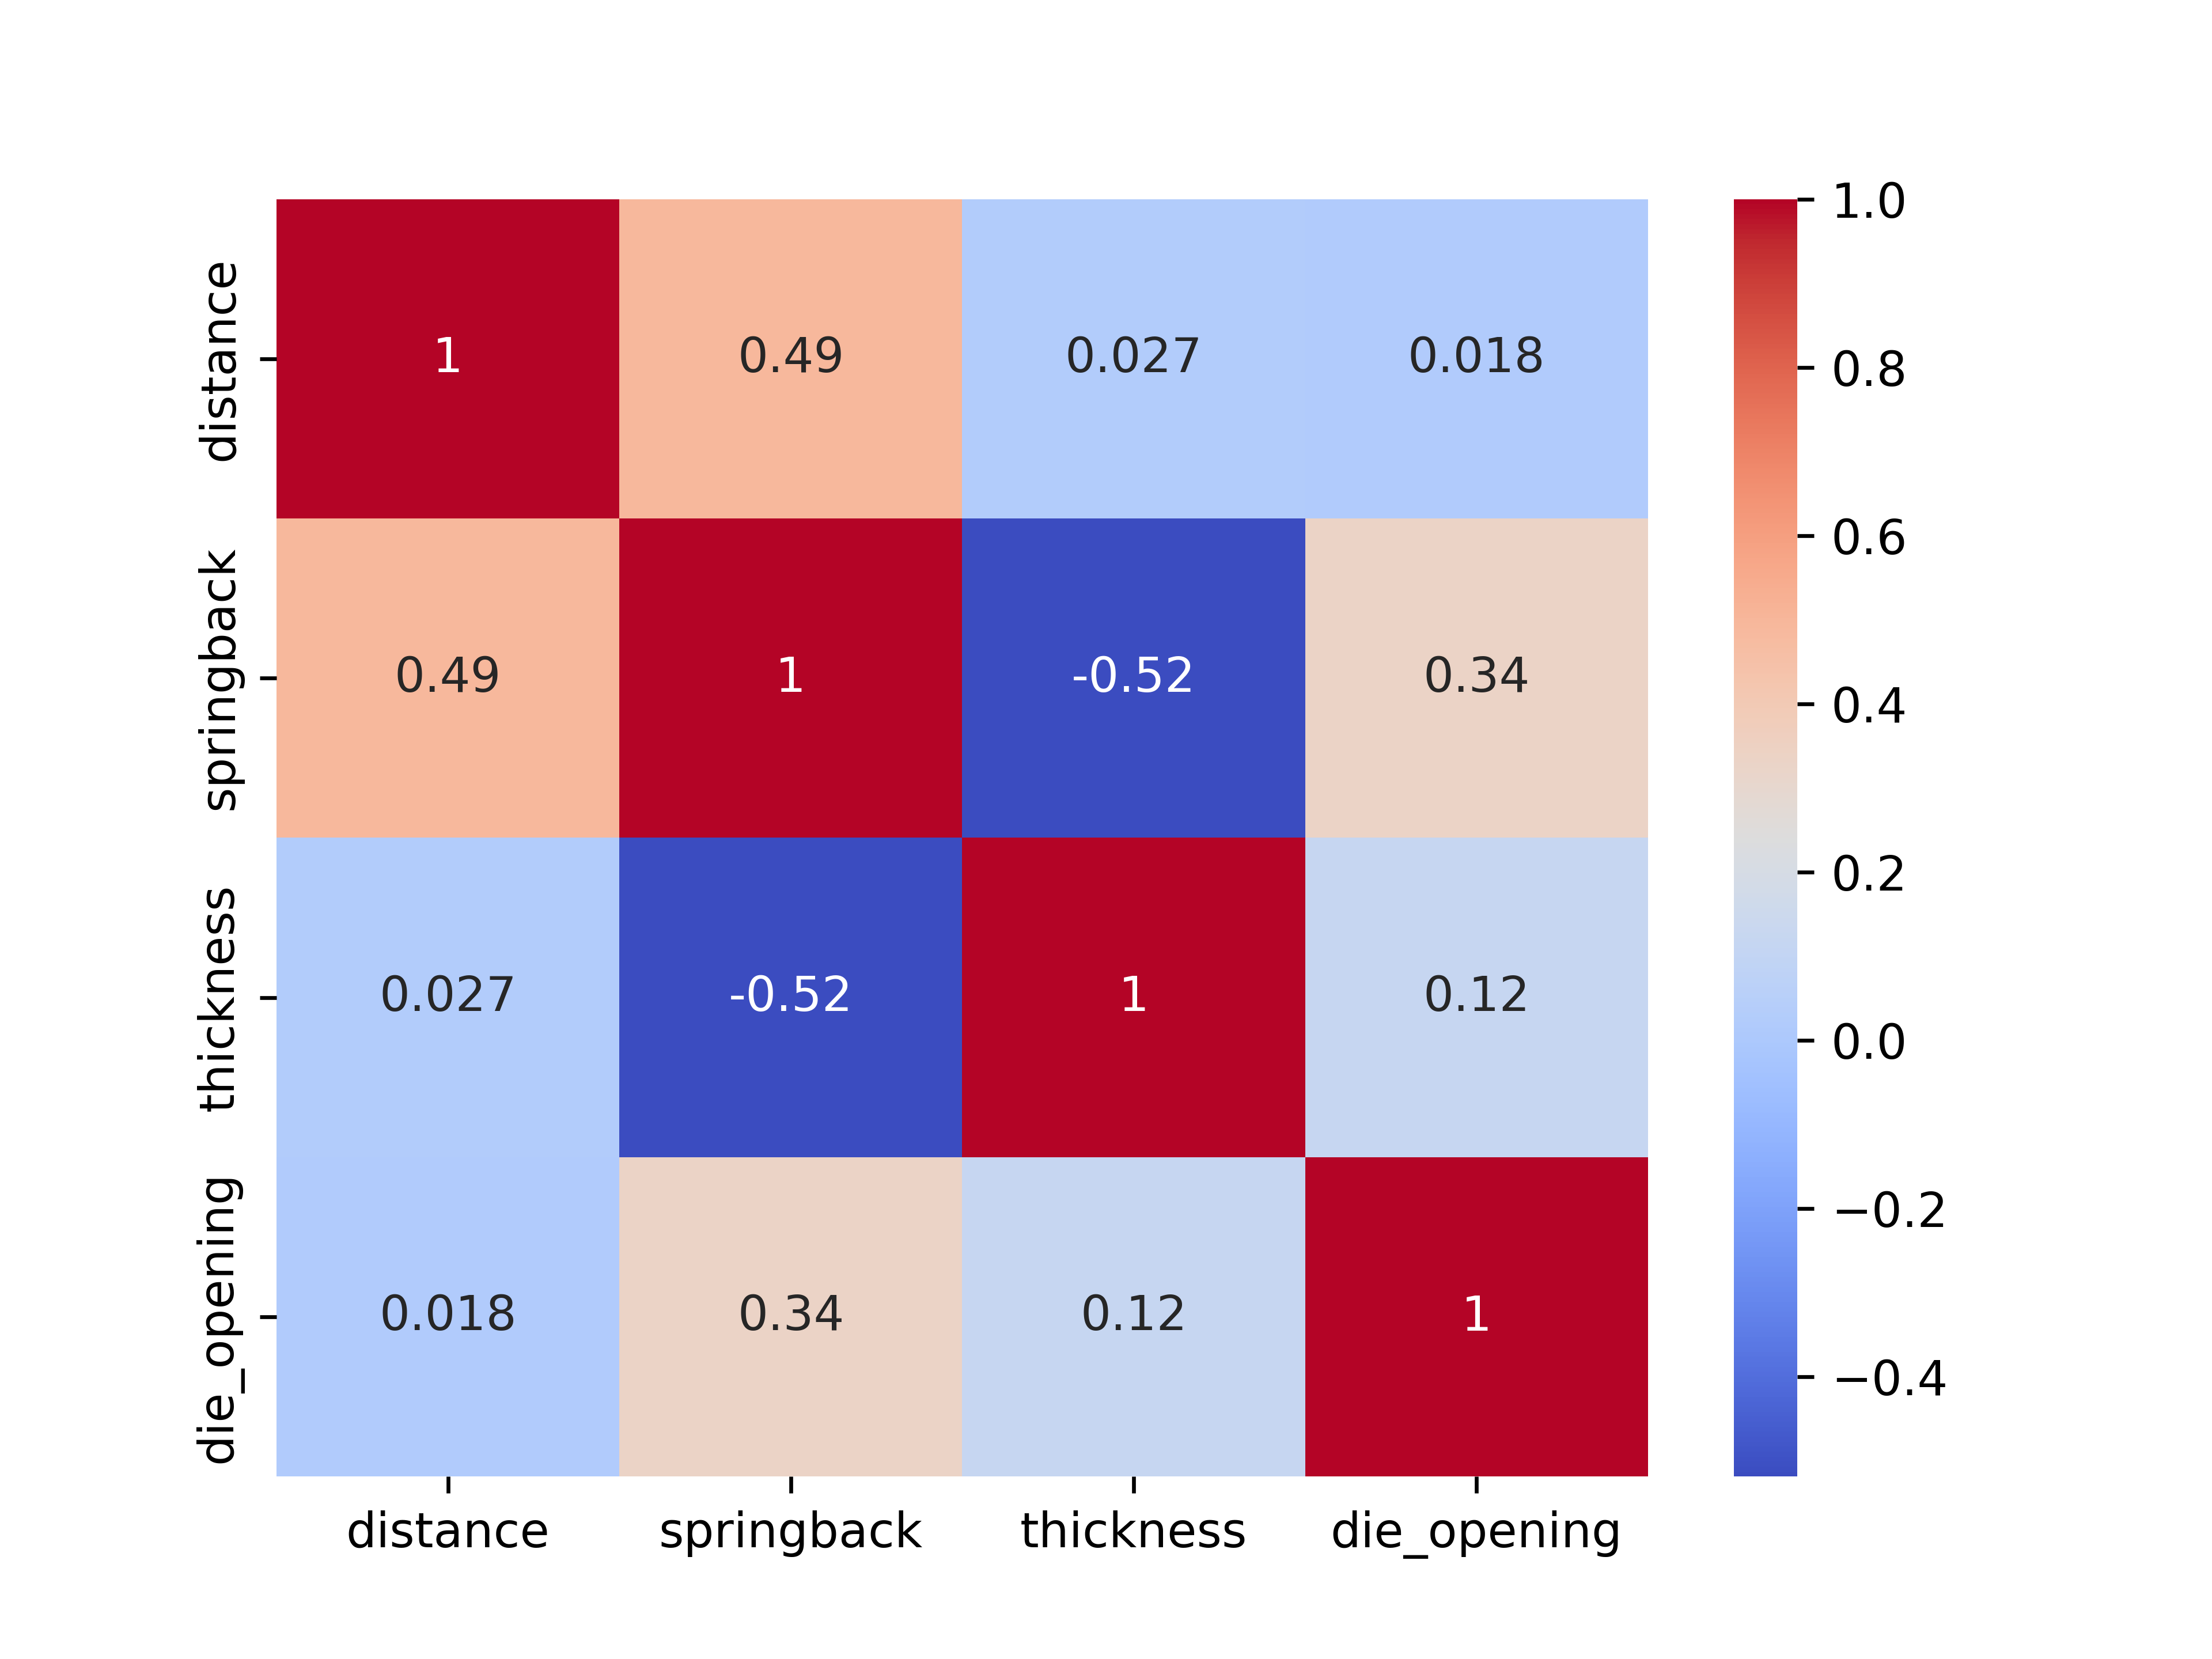
\includegraphics[width=0.9\textwidth]{correlation_matrix}
    \caption{Correlation matrix}
    \label{fig:correlation_matrix}
\end{figure}

\section{Model Selection}
\subsection{Support Vector Regression (SVR)}
Support Vector Machines \ac{SVM} are used for classification problems. The \ac{SVM} algorithm is used to find a hyperplane in an N-dimensional space (N - the number of features) that distinctly classifies the data points. \cite[p. 42]{awad_efficientlearningmachines_2015}
Predicting the spring back is a regression problem, so the \ac{SVM} algorithm is not suitable for this problem. It therefore is a generalization of classification problems, where the model returns continuous values instead of finite set of values.
The Support Vector Regression \ac{SVR} algorithm is derived from the \ac{SVM} algorithm and accomblishes this generalization by introducing an $\epsilon$-intensive region around the function ($\epsilon-tube$).  \cite[p. 67]{awad_efficientlearningmachines_2015}

\subsection{Multi Linear Regression}
\subsection{Polynomial Regression}
\subsection{Decision Tree Regression}
\subsection{Random Forest Regression}
% Erst einmal auf decision tree generell eingehen
A commonly used method in machine learning. The goal is to solve classification or regression problems by predicting the value of a output variable by one or multiple input variables. \cite[p. 253]{shaik_briefsurveyrandom_2019}
To build a \ac{DT} the source dataset represents the root node of the tree this data set is split into leafs (children) by using a set of spitting rules until each leaf in the \ac{DT} is "pure" and only contains one target value. Depending on the use cases this is a single class or a single regression value. \cite[p. 70-72]{muller_introductionmachinelearning_2016}
% -> Problem von decision tree 
The main drawbback of \ac{DT}s is the tendency to overfit and poor generalization performance, what makes them not paticaly for most use cases. Therefore usualy ensemble methods are used instead of a single \ac{DT}. \cite[p. 78]{muller_introductionmachinelearning_2016} \cite[p. 251]{liu_newmachinelearning_2012}
% -> Warum random forst das problem löst 
Random forest \cite[]{breiman_randomforests_2001} is a type of ensemble learning algorithm in which multiple decision trees, which are "weak learners," are trained and combined to produce a more accurate and stable prediction, known as a "strong learner." \cite[p. 24]{awad_efficientlearningmachines_2015}
The risk of overfitting is mitigated by subset and feature randomization. Each root node uses a unique subset of the data and each leaf is split using a random features. This ensures that no single tree sees all of the data, allowing the model to focus on general patterns rather than being sensitive to noise. \cite[p. 251]{liu_newmachinelearning_2012}
% -> Beschreibung Random forest / Random foret regression 
In this supervised learning method,
%which was influenced by the research of Amit and Geman (1997), Ho (1998), and Dietterich (2000), 
a "divide and conquer" approach is used. This involves dividing the data into smaller samples, incrementally building a randomized tree predictor for each sample, and then combining (aggregating) these predictors together. This approach has proven to be effective. Because not only one but multiple classifiers are used the random forest learning is known as ensemble model. \cite[p. 254]{shaik_briefsurveyrandom_2019}

% -> Vorteile / Nachteile Random Forest 
This mechanism is flexible enough to handle classifications and regression problems, this is one of the reasons that random forests count to the most successful \ac{ML} methods. \cite[p. 3-4]{biau_randomforestguided_2016} \cite[p. 25]{breiman_randomforests_2001}

%
% Advantages
%
Random forests are a type of machine learning algorithm that uses bagging and the random selection of features to produce accurate results. They are effective at handling noise and can work with both continuous and categorical variables. This combination of techniques helps improve the performance of the algorithm. \cite[p. 259]{liu_newmachinelearning_2012}
Decision trees have a limitation in their ability to overfit, which is a disadvantage. This is mitigated by the use of subset and feature randomization. Specifically, each base model uses a unique subset of the data, and each node in the decision tree is split using a random set of features. This ensures that no single tree sees all of the data, allowing the model to focus on general patterns rather than being sensitive to noise. \cite[p. 259]{liu_newmachinelearning_2012}

% Bagging technique helps the algorithms performance. 
% Works well out of the box with no hyperparameter tuning.
% Fast, robust, and can show feature importances which can be quite useful.

% Disadvantages
%

% Boosted algos usuallaly outperform Random Forest.
% RF is not able to extrapolate based on the data. It can only predict within the range of the training data.
% Random forest regressor is unalbe to discover trens that would enable it in extrapolating values that fall outside of the training set.   

%  Extrapolating is the process of estimating or predicting something beyond the range of available data. (chatgpt)

%
% Alogithm steps 
%

% The following Random Forest Algorithm [9] gives the steps in constructing the
% decision trees.
% • Take N as the number of training data instances in the samples. Let M be the
% number of attributes in given input dataset.
% • Let m be the Number of parameter in the input that determines the next attribute
% to be chosen at each tree node; (where mislesserthan M).
% • The training samples are taken and a tree is constructed for each sample with
% replacement.
% • For tree node, arbitrarily select m attributes in that particular node.
% • The best split is computed based on the m input attributes of the sample dataset.
% • Each tree is grown without pruning.
% \cite[p. 254-255]{shaik_briefsurveyrandom_2019}

% A random forest does not require any cross verification and it is not over-fitting [8]. The
% Random forest uses Adaboost and Bootstrapping techniques to construct multiple
% classifiers. \cite[p. 254]{shaik_briefsurveyrandom_2019} 


% In a classification random forest, each tree in the forest makes a prediction for the class label of a given example, and the final prediction is made by majority vote, with the class label that receives the most votes being chosen as the prediction. In a regression random forest, each tree in the forest makes a prediction for the continuous value, and the final prediction is made by averaging the predictions of all the trees in the forest. (chatgpt)

% In both cases, the random forest model creates a large number of decision trees and trains them on different subsets of the training data. The decision trees are trained using a technique called bagging, which involves randomly selecting a subset of the training examples for each tree and training the tree on that subset. The idea behind bagging is to train each tree on a slightly different subset of the data, which can help to reduce overfitting and improve the overall performance of the model. (chat gpt)

\subsubsection*{Results}

\section{Model Training}


\subsection{Training-Test Split}
Figure~\ref{fig:train_test_split} shows the data set and which parts of it is used for training and testing the used models. Samples with a die opening of 30 are used to test the performance and the remaining part is used for training. 
A different approach would be to us a random test and train split, this would lead to a better performance of the models but would not evaluate their ability to predict new data of a different die opening.
The die opening 30 was chosen because it is in the middle of the selected data set and therefore the models should be able to predict the data of this die opening.
All models are trained with the same data set and the same parameters. The only difference is the used algorithm.


\begin{figure}[H]
    \centering
    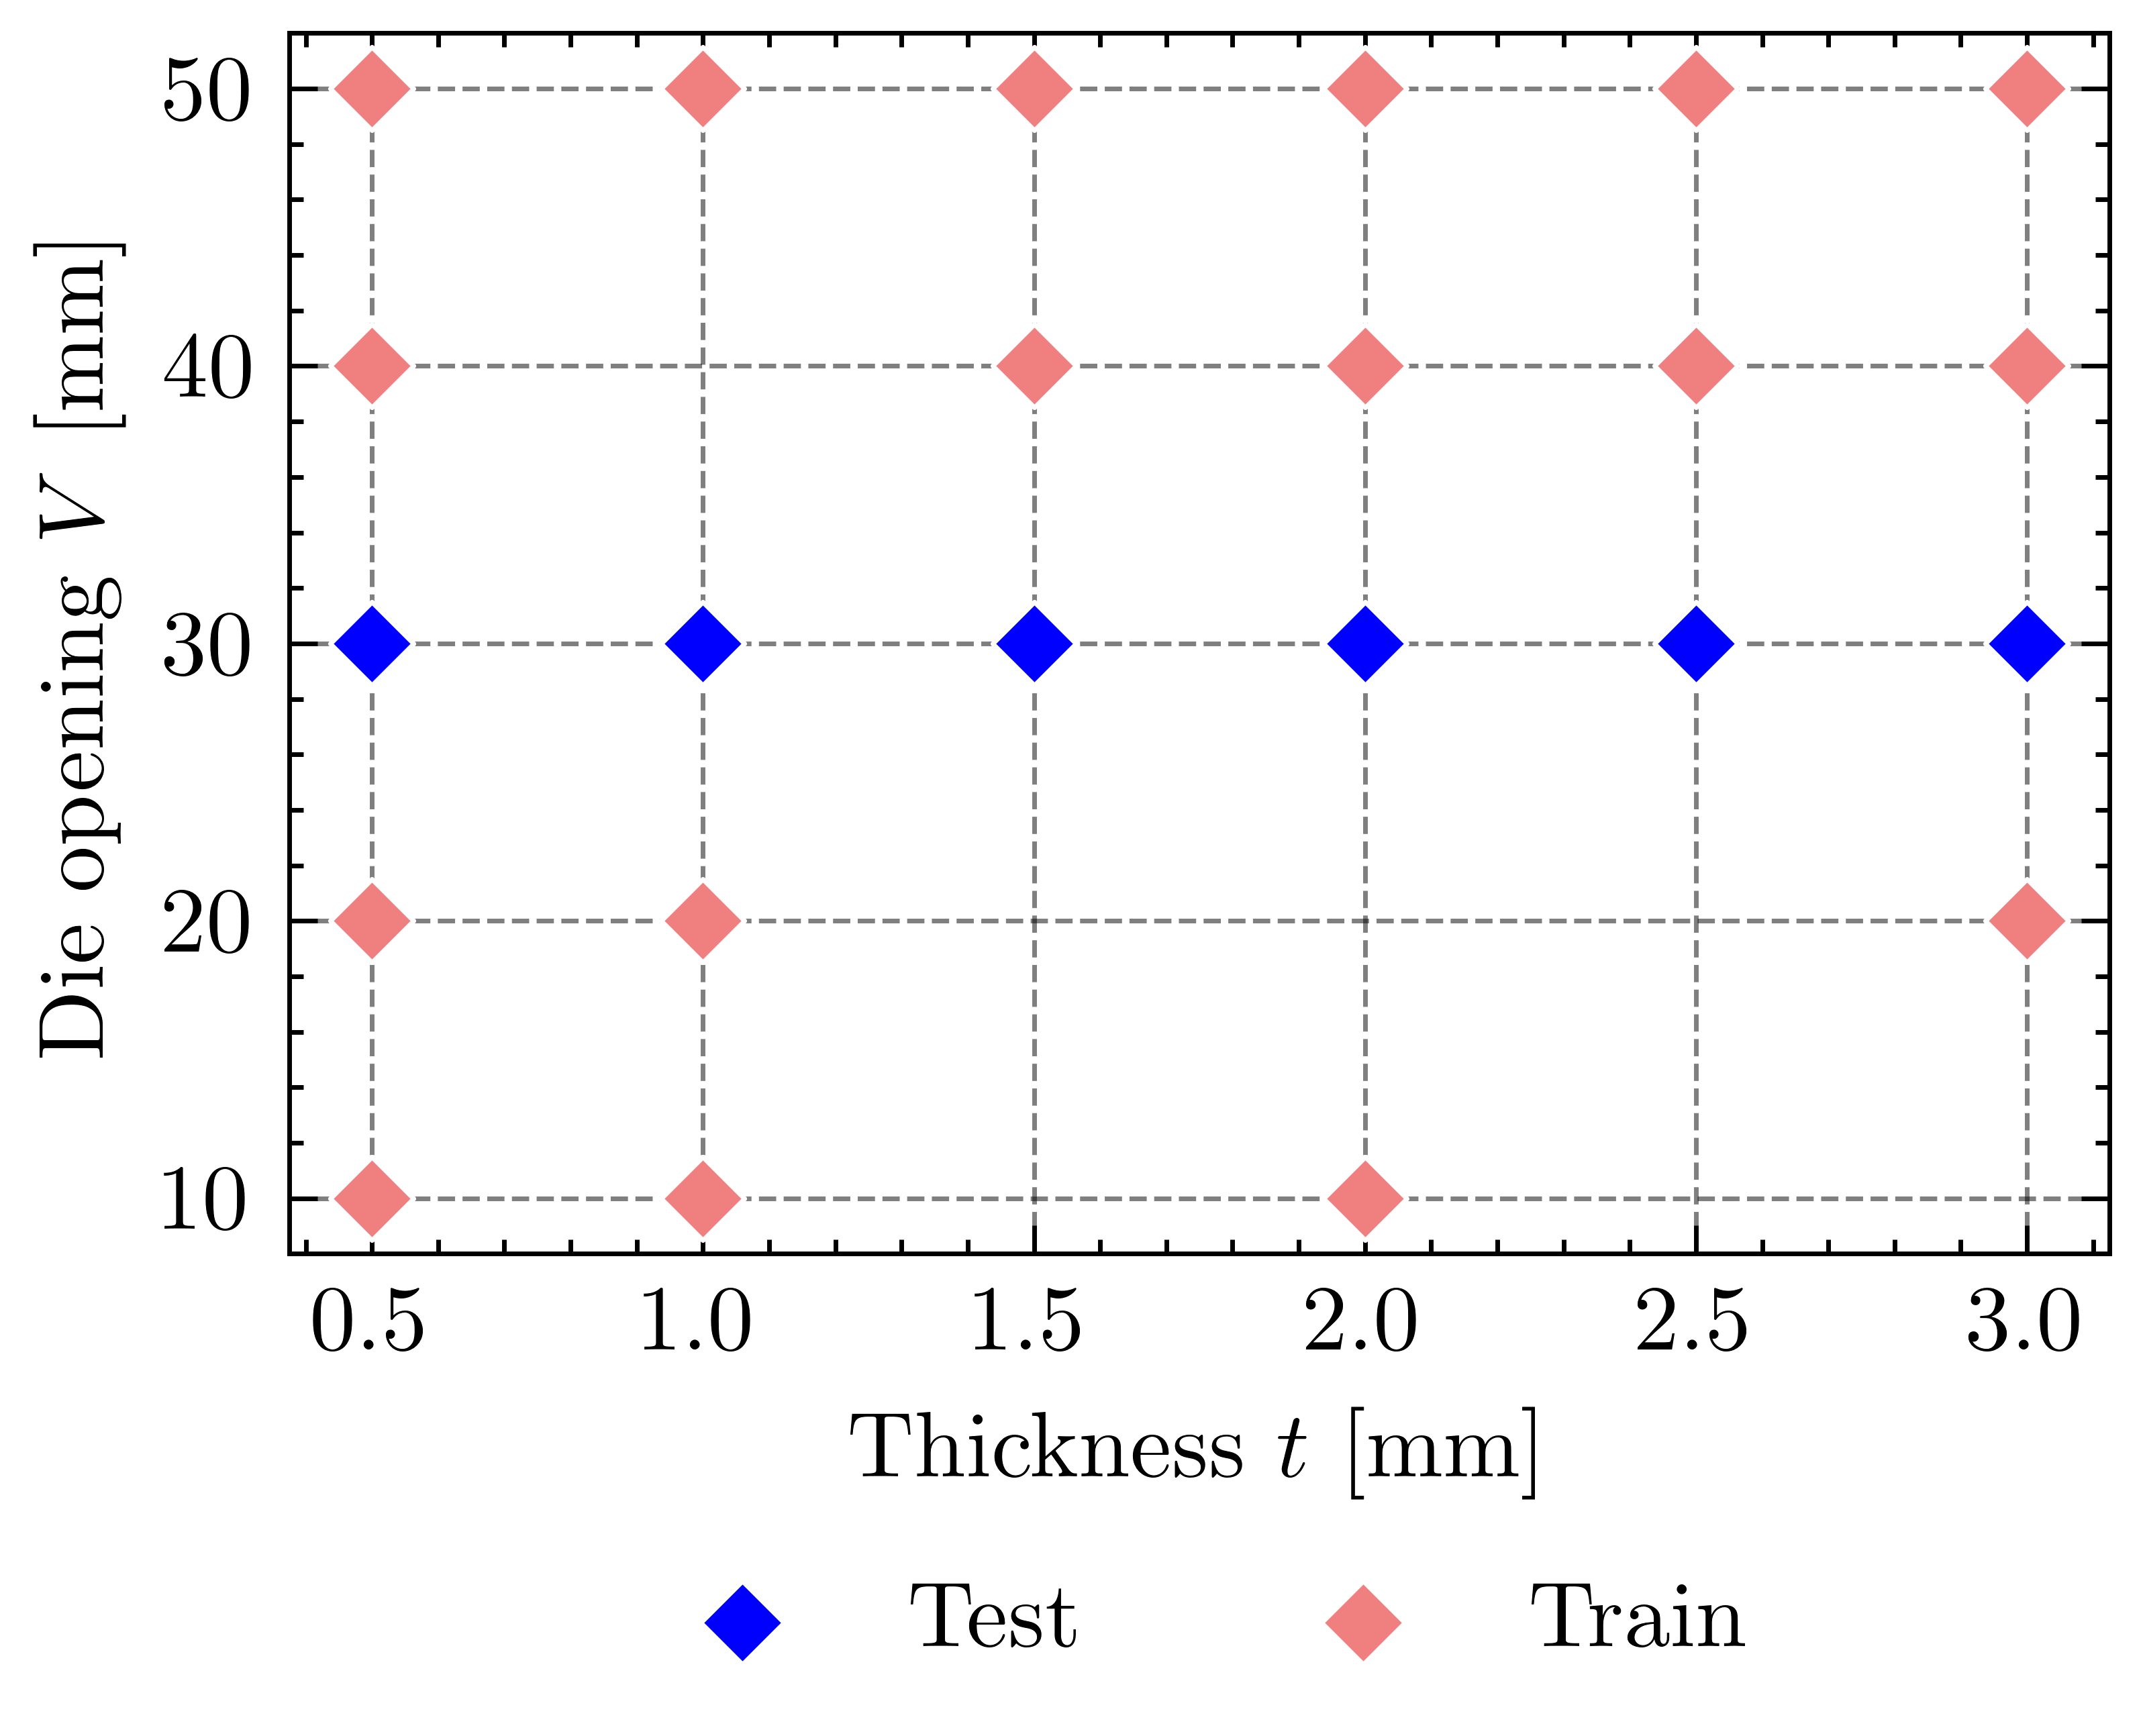
\includegraphics[width=1\textwidth]{test_train_split}
    \caption{The training and test dataset. (Data especially for V40 is still missing)}
    \label{fig:train_test_split}
\end{figure}

\subsubsection*{Tuning}
bootstrap: true, criterion: squared error, min samples leaf : 1, min samples split: 2, max features: 0.5119924258446656, n estimators: 35, n jobs: -1.










% \paragraph{Bend deduction:}
% Measuring the bend deduction is more complex. After a metal sheet is bent, it is hard to measure the flat pattern length because the material is malformed at the bent. 
% As a result, the neutral axis is not in the center of the sheet and hard to measure, but it can be calculated using different approaches. %quelle und ausführlicher und grunlagen teil  
% There are multiple ways to measure the bend deduction described earlier. 
% % K-Faktor Muss noch in theorie teil 
% In this setup, the method described in the DIN6395 was used. This method uses a k-factor which is an approximated value and therefore and therefore it can be inaccurate. (Equation~\ref{eq:kfactor}). % cite DIN norm 

% \begin{equation}\label{eq:kfactor}
%     k=0.65+\frac{1}{2}\log{\frac{r}{s}}
% \end{equation}

% \begin{figure}[ht!] % supposedly places it here ...
% 	\centering
% 	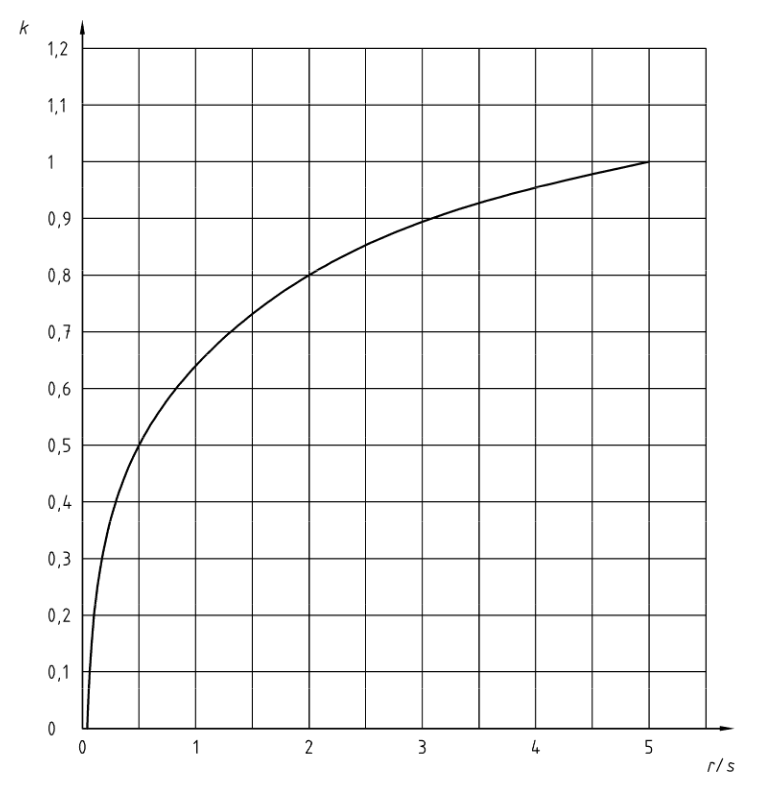
\includegraphics[width=0.5\linewidth]{k-factor}
% 	\caption[Graphical representation of the correction factor]{Graphical representation of the correction factor.}
% 	\label{fig:test1}
% \end{figure}

% The DIN 6935 used the formula for the stretched length, $length=a+b+v$ where \textit{a} and \textit{b} are the side lengths of the sheet and \textit{v} is a correction value for the deduction. \cite{din6935}
% The stretched length is measured different depending on the bending angle.

% \paragraph{Opening angle $\beta 0^\circ$ to $90^\circ$} 
% For opening angles between $0^\circ$and $90^\circ$ the side lengths \textit{a} and \textit{b} are dimensioned from the tangent of the bend to the edge. 
% To calculate the compensation value \textit{v} (Equation~\ref{eq:v1}) is used
% \cite{din6935}.

% \begin{equation}\label{eq:v1}
%         v=\pi*(\frac{180^\circ-}{180^\circ})*(r+\frac{s}{2}*k)-2(r+s)
% \end{equation}

% \begin{figure}[H]
% 	\centering
% 	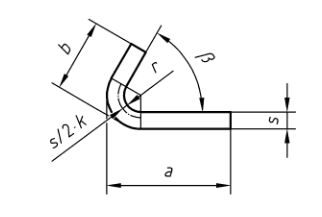
\includegraphics[width=0.5\linewidth]{bending-angle-90}
% 	\caption[Opening angles $\beta 0^\circ$ to $90^\circ$]{Opening angles $\beta 0^\circ$ to $90^\circ$ \cite{din6935}}
% 	\label{fig:v1-image}
% \end{figure}

% \paragraph{Bending angle $\beta90^\circ$ to $165^\circ$} (Equation~\ref{eq:v1})
% For opening angles between $90^\circ$ and $165^\circ$ the side lengths \textit{a} and \textit{b} are dimensioned from the apex to the edge. 
% To calculate the compensation value \textit{v} (Equation~\ref{eq:v1}) is used. 
% \cite{din6935}

% \begin{equation}\label{eq:v2}
%     v=\pi*(\frac{180^\circ-}{180^\circ})*(r+\frac{s}{2}*k)-2(r+s)+\tan{\frac{180^\circ-\beta}{2}}
% \end{equation}

% \begin{figure}[!ht]
% 	\centering
% 	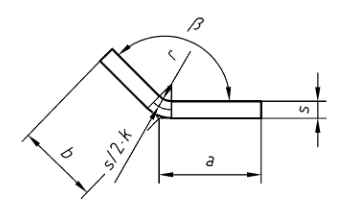
\includegraphics[width=0.5\linewidth]{bending-angle-165}
% 	\caption[Opening angles $\beta90^\circ$ to $165^\circ$]{Opening angles $\beta90^\circ$ to $165^\circ$ \cite{din6935}}
% 	\label{fig:v2-image}
% \end{figure}

% For opening angles between $165^\circ$ and $180^\circ$ the compensation value \textit{v} is 0. The values for v would be negligibly small. \cite{din6935} The side lengths \textit{a} and \textit{b} where measured using the software \textit{ImageJ}. 

% Edge cracking is not measured for now because the steel used has no high-strength and with machine in usage it was not possible to create edge cracking.

% \begin{figure}[!ht]
% 	\centering
% 	\includegraphics[width=0.5\linewidth]{example-image}
% 	\caption[Screenshot ImageJ]{Screenshot ImageJ}
% 	\label{fig:imagej-screenshot}
% \end{figure}

